% ************************************************************************
\documentclass[12pt,oneside,letterpaper]{article}
% ************************************************************************

\usepackage[small,bf]{caption}
\renewcommand{\thefigure}{S\arabic{figure}}
\usepackage{cite}
\usepackage{times}
\usepackage{helvet}
\usepackage{epsf}
\usepackage{graphicx}
\usepackage{graphbox}
\usepackage{amsmath}
\usepackage[mathscr]{euscript}
\usepackage{algorithm}
\usepackage{algpseudocode}
%\usepackage{multirow}

% ************************************************************************

\columnsep        0.0in
\evensidemargin   0.0in
\footskip         0.2in
\headheight       0.3in
\headsep          0.3in
\hoffset          0.0in
\marginparpush    0.0in
\marginparsep     0.0in
\marginparwidth   0.0in
\oddsidemargin    0.0in
\paperheight     11.0in
\paperwidth       8.5in
\tabcolsep        0.0in
\textheight       8.8in
\textwidth        6.5in
\topmargin        0.0in
\voffset         -0.25in
\parindent        0.0em
\parskip          0.0em

% ************************************************************************

\usepackage{fancyhdr}
\pagestyle{fancyplain}
\renewcommand{\sectionmark}[1]{}{}
\renewcommand{\subsectionmark}[1]{}
\lhead[\fancyplain{}{}]{\fancyplain{}{}}
\chead[\fancyplain{}{}]{\fancyplain{}{}}
\rhead[\fancyplain{}{}]{\fancyplain{}{}}
\lfoot[\fancyplain{}{}]{\fancyplain{}{}}
\cfoot[\fancyplain{}{}]{\fancyplain{}{\thepage}}
\rfoot[\fancyplain{}{}]{\fancyplain{}{}}
\renewcommand{\headrulewidth}{0pt}
\renewcommand{\footrulewidth}{0pt}

% ************************************************************************
\begin{document}
% ************************************************************************

\thispagestyle{empty}

\begin{center}

\vspace*{10\baselineskip}

{\huge\sffamily Automated neuron tracing using\\[0.5em] probability hypothesis density filtering}

\vspace{2\baselineskip}

{\large Miroslav Radojevi{\'c} and Erik Meijering}

\vspace{2\baselineskip}

{\large\bfseries Supplementary Information}

\end{center}

% ************************************************************************
\renewcommand{\baselinestretch}{1.5}
% ************************************************************************
\clearpage
\vspace*{8\baselineskip}
\begin{algorithm}
\caption{Neuron tracing}\label{alg:delin}
\begin{algorithmic}[1]
\State{}{$k=0$}\Comment{Initialize}
\State{}{$\lbrace \omega_{0|0}^n, \mathrm{x}_{0|0}^n \rbrace_{n=1}^{\rho N_0}$}\Comment{Initial particle and observation set}
\State{}{$\lbrace \hat{\mathrm{x}}_{0,i} \rbrace_{i=1}^{N_{0}}$}\Comment{Initial estimate}
\Repeat
\State{}{$k=k+1$}
\State{}{$\mathrm{p}_{i}^{n} \sim h(\mathrm{p} | \hat{\mathrm{x}}_{k-1,i}) \quad n \in \left[ 1, \rho N_{k-1}\right]$}\Comment{Draw observation particles} \label{alg:line:draw-obs-particles} 
\State{}{$\mathrm{p}_{i,j}^n \in \mathscr{C}_j , \quad j \in \left[ 1, M_k \right], \quad n \in \left[ 1, |\mathscr{C}_j| \right]$}\Comment{Cluster observation particles}
\State{}{$\mathrm{z}_{k,j} = \left[ \mathrm{p}_{i,j}^{\hat{n}}, \tau(\mathrm{p}_{i,j}^{\hat{n}}) \right]$}\Comment{Select representative sample} \label{alg:line:construct-obs} 
\State{}{$\mathrm{Z}_{k} = \lbrace \mathrm{z}_{k,j},\dots, \mathrm{z}_{k,M_k}  \rbrace$}\Comment{Construct observations}
\State{}{$\lbrace \omega_{k|k}^n, \mathrm{x}_{k|k}^n \rbrace_{n=1}^{\rho N_{k}}, \nu_{k}, \lbrace \hat{\mathrm{x}}_{k,i} \rbrace_{i=1}^{N_k} \leftarrow$ SMC-PHD$(\lbrace \omega_{k-1|k-1}^n, \mathrm{x}_{k-1|k-1}^n \rbrace_{n=1}^{\rho N_{k-1}}, \mathrm{Z}_{k})$}\Comment{Algorithm~\ref{alg:smc-phd}}
\Until{$\left[ \nu_{k} \right] = 0$} \Comment{$\left[ \cdot \right] \equiv $ nearest integer}
\end{algorithmic}
\end{algorithm}

% ************************************************************************
\clearpage
\vspace*{3\baselineskip}
\begin{algorithm}
\caption{SMC-PHD filtering}\label{alg:smc-phd}
\begin{algorithmic}[1]
\State{Input:}{$\lbrace ( \omega_{k-1|k-1}^n, \mathrm{x}_{k-1|k-1}^n ) \rbrace_{n=1}^{\rho N_{k-1}}, \lbrace \mathrm{z}_{k,j}  \rbrace_{j=1}^{M_k}$}
\Comment{$D_{k-1}(\mathrm{x})$ approx. observation $\mathrm{Z}_k$}
\For{$n=1,\dots,\rho N_{k-1}$} 
\For{$m=1,\dots,\eta$}
\State{}{$i = (n-1)\eta+m$}
\State{Draw: }{$\mathrm{x}_{k|k-1,\mathrm{p}} \sim \pi_{k|k-1}(\mathrm{x}|\mathrm{x}_{k-1|k-1}^{n}) \rightarrow \mathrm{x}_{k|k-1,\mathrm{p}}^{i}$}\Comment{Persistent object particles} \label{alg:line:pred-p} 
\State{Compute: }{$\omega_{k|k-1, \mathrm{p}}^{i} = p_S \tfrac{1}{\eta} \omega_{k-1|k-1}^{n}$}
\State{Draw: }{$\mathrm{x}_{k|k-1,\mathrm{s}} \sim \beta_{k|k-1}(\mathrm{x}|\mathrm{x}_{k-1|k-1}^{n}) \rightarrow \mathrm{x}_{k|k-1,\mathrm{s}}^{i}$}\Comment{Spawning object particles} \label{alg:line:pred-s} 
\State{Compute: }{$\omega_{k|k-1, \mathrm{s}}^{i} = p_S \tfrac{1}{\eta} \omega_{k-1|k-1}^{n}$}
\EndFor
\EndFor
\State{$\lbrace(\omega_{k|k-1}^n, \mathrm{x}_{k|k-1}^n)\rbrace_{n=1}^{S_k} = \lbrace(\omega_{k|k-1,\mathrm{p}}^n, \mathrm{x}_{k|k-1,\mathrm{p}}^n)\rbrace_{n=1}^{\rho \eta N_{k-1}} \cup \lbrace(\omega_{k|k-1,\mathrm{s}}^n, \mathrm{x}_{k|k-1,\mathrm{s}}^n)\rbrace_{n=1}^{\rho \eta N_{k-1}}$}{} \Comment{Union of particle sets}
\For{$n=1,\dots,S_k$} % \limits
\State{Update: }{$\omega_{k|k}^n = (1-p_D)\omega_{k|k-1}^n+\sum\limits_{\mathrm{z} \in \mathrm{Z}_k}\tfrac{p_D g_k(\mathrm{z}|\mathrm{x}_{k|k-1}^n) \omega_{k|k-1}^n}{C_k(\mathrm{z}) + \sum_{n=1}^{S_k}p_D g_k(\mathrm{z}|\mathrm{x}_{k|k-1}^n)\omega_{k|k-1}^n }$}\label{alg:line:particle-update}
\EndFor
\State{}{$\nu_k = \sum\limits_{n=1}^{S_{k}} \omega_{k|k}^n$} \Comment{Cardinality calculation}
%\State{}{$N_{k} = \rho$} \Comment{}
\State{Estimate: }{$\hat{\mathrm{x}}_{k,i} \leftarrow \lbrace  \omega_{k|k}^n, \mathrm{x}_{k|k-1}^n  \rbrace_{n=1}^{S_k}$}\Comment{Mean-shift clustering}
% $N_k$ times 
\State{Resample: }{$N_k=\left[ \nu_k \right], \lbrace  \omega_{k|k}^n  , \mathrm{x}_{k|k-1}^n  \rbrace_{n=1}^{S_k} \rightarrow \lbrace \omega_{k|k}^n ,  \mathrm{x}_{k|k}^n\rbrace_{n=1}^{\rho N_k}, \omega_{k|k}^n = \nu_k / (\rho N_k) $\\} \Comment{Systematic resampling with $\rho$ particles per object}
\end{algorithmic}
\end{algorithm}

% ************************************************************************
\clearpage
\begin{figure}[!t]
\centering
\begin{tabular}{c@{\hspace{1em}}c@{\hspace{1em}}c}
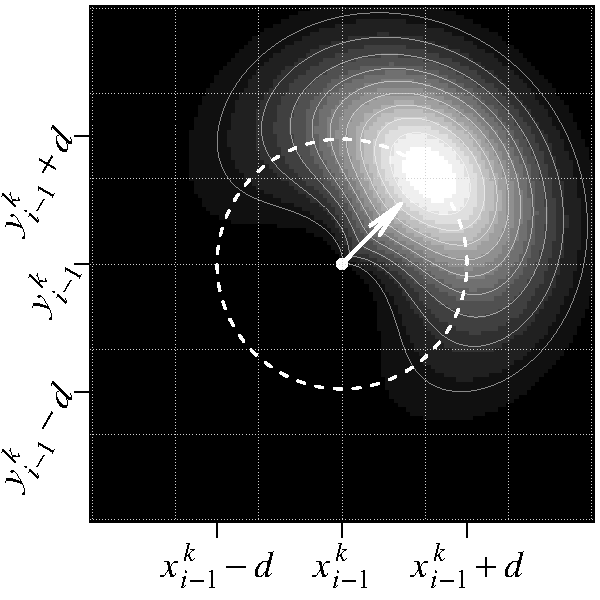
\includegraphics[height=0.3\columnwidth]{./fig/pi} &
\includegraphics[height=0.3\columnwidth]{./fig/beta} &
\includegraphics[height=0.3\columnwidth]{./fig/h} \\
(A) $\pi_{k|k-1}(\mathrm{x}|\mathrm{x'})$ & (B) $\beta_{k|k-1}(\mathrm{x}|\mathrm{x'})$ & (C) $h(\mathrm{p}|\mathrm{x'})$ \\
\end{tabular}  		
\caption{Transition densities (2D examples) for persistent (A) and spawned (B) objects with $z=0$, $\mathrm{x'}=\left[ 0,0,0, \tfrac{1}{\sqrt{2}},\tfrac{1}{\sqrt{2}}, 0 \right] $, $\kappa=2$, and $r_k=3$. (C) Importance sampling used in the observation model without the tubularity component, $\tau(\mathrm{p})=1$, and $\kappa=0.5$. Rainbow color coding is used running from blue (indicating low values) to red (indicating high values).}
\label{fig:transitions}
\end{figure}

% ************************************************************************
\clearpage
\begin{figure}[!t]
\centering
\begin{tabular}{c@{\hspace{2em}}c}
\includegraphics[width=0.4\columnwidth]{./fig/o1} &
\includegraphics[width=0.4\columnwidth]{./fig/o2} \\[-1ex]
(A) $\mathrm{p}_{i}^{n} \sim h(\mathrm{p} | \hat{\mathrm{x}}_{k-1,i})$ &
(B) $\mathrm{p}_{i,j}^n \in \mathscr{C}_j$ \\[3ex]
\includegraphics[width=0.4\columnwidth]{./fig/o3} &
\includegraphics[width=0.4\columnwidth]{./fig/Cz} \\[-1ex]
(C) $\mathrm{z}_{k,j}$ &
(D) $C_k(\mathrm{z}) = e^{-K_c\tau_{\mathrm{z}}}$ 
\end{tabular}
\caption{Formation of the observations (2D example). (A) For each object $i$ from iteration $k-1$, particles $\mathrm{p}_{i}^{n}$ are sampled from the importance sampling function $h$, using the state estimate $\hat{\mathrm{x}}_{k-1,i}$. The solid dot indicates the location of $\hat{\mathrm{x}}_{k-1,i}$ and the contours represent lines of equal particle weight. (B) The particles are processed by mean-shifting resulting in clusters $\mathscr{C}_j$ whose labeled particles are denoted as $\mathrm{p}_{i,j}^{n}$. (C) Each observation $\mathrm{z}_{k,j}$ is obtained from the representative cluster particle $\mathrm{p}_{i,j}^{\hat{n}}$ as described in the main text. Contours represent lines of equal observation likelihood. (D) The clutter intensity function.} 
\label{fig:observation-model}
\end{figure}

% ************************************************************************
\clearpage
\begin{figure}[!t]
\centering
\begin{tabular}{c@{\hspace{1ex}}c@{\hspace{1ex}}c@{\hspace{3ex}}c@{\hspace{1ex}}c@{\hspace{1ex}}c}
(A) &
\includegraphics[align=c,width=0.2\columnwidth]{./fig/101_accno} &% ./fig/opfA/101/acc[no]
\includegraphics[align=c,width=0.2\columnwidth]{./fig/101_accround3} &% ./fig/opfB/101/acc[round]3
(B) &
\includegraphics[align=c,width=0.2\columnwidth]{./fig/109_accno} &% ./fig/opfA/109/acc[no]
\includegraphics[align=c,width=0.2\columnwidth]{./fig/109_accround3} \\% ./fig/opfB/109/acc[round]3
\vspace{-2ex} \\
(C) &
\includegraphics[align=c,width=0.2\columnwidth]{./fig/104_accno} &% ./fig/opfA/104/acc[no]
\includegraphics[align=c,width=0.2\columnwidth]{./fig/104_accround3} &%./fig/opfB/104/acc[round]3
(D) &
\includegraphics[align=c,width=0.2\columnwidth]{./fig/106_accno} &% ./fig/opfA/106/acc[no]
\includegraphics[align=c,width=0.2\columnwidth]{./fig/106_accround3} \\% ./fig/opfB/106/acc[round]3
\vspace{-2ex} \\
(E) &
\includegraphics[align=c,width=0.2\columnwidth]{./fig/301_accno} &% ./fig/sariaA/301/acc[no]
\includegraphics[align=c,width=0.2\columnwidth]{./fig/301_accround} &% ./fig/sariaB/301/acc[round]
(F) &
\includegraphics[align=c,width=0.2\columnwidth]{./fig/302_accno} &% ./fig/sariaA/302/acc[no]
\includegraphics[align=c,width=0.2\columnwidth]{./fig/302_accround} \\% ./fig/sariaB/302/acc[round]
\vspace{-2ex} \\
(G) &
\includegraphics[align=c,width=0.2\columnwidth]{./fig/305_accno} &% ./fig/sariaA/305/acc[no]
\includegraphics[align=c,width=0.2\columnwidth]{./fig/305_accround} &% ./fig/sariaB/305/acc[round]
(H) &
\includegraphics[align=c,width=0.2\columnwidth]{./fig/306_accno} &% ./fig/sariaA/306/acc[no]
\includegraphics[align=c,width=0.2\columnwidth]{./fig/306_accround} \\% ./fig/sariaB/306/acc[round]
\end{tabular}
\caption{Performance as a function of numbers of seeds and rounds for four example cases from the OPF (A-D) and the HCN (E-H) data set. Similar trends were observed for all cases in the respective data sets. Left panel per case: Precision (P), recall (R), and F-score (F) after one round initialized with different numbers of seeds ($N_0$). Right panel per case: The scores after multiple rounds with a fixed number of seeds ($N_0=40$). Fifth-order polynomial curves were fit to the data to show approximate trends.}
\label{fig:opf-saria-tests}
\end{figure}

% ************************************************************************
\clearpage
\begin{figure}[!t]
\centering
\begin{tabular}{c@{\hspace{0.02\columnwidth}}c@{\hspace{0.02\columnwidth}}c}
\includegraphics[width=0.31\columnwidth]{./fig/p_opf} &% ./fig/compare/opf/p
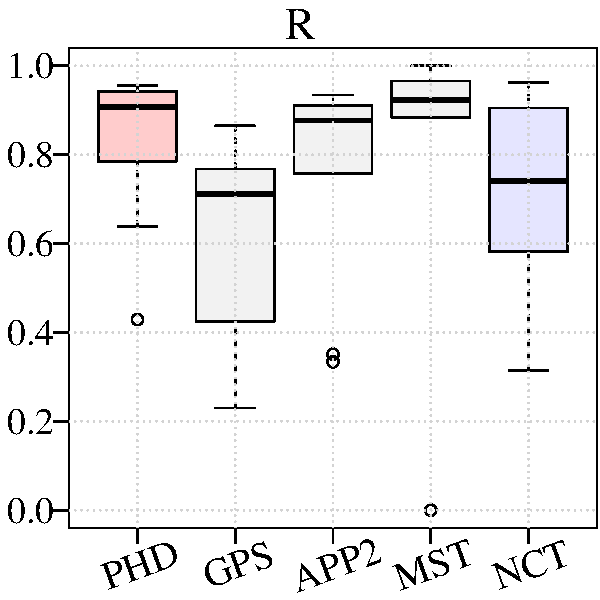
\includegraphics[width=0.31\columnwidth]{./fig/r_opf} &% ./fig/compare/opf/r
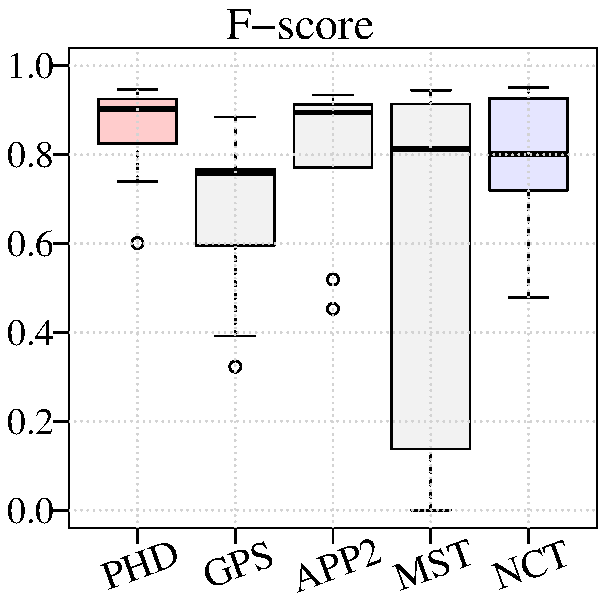
\includegraphics[width=0.31\columnwidth]{./fig/f_opf} \\[1ex]% ./fig/compare/opf/f
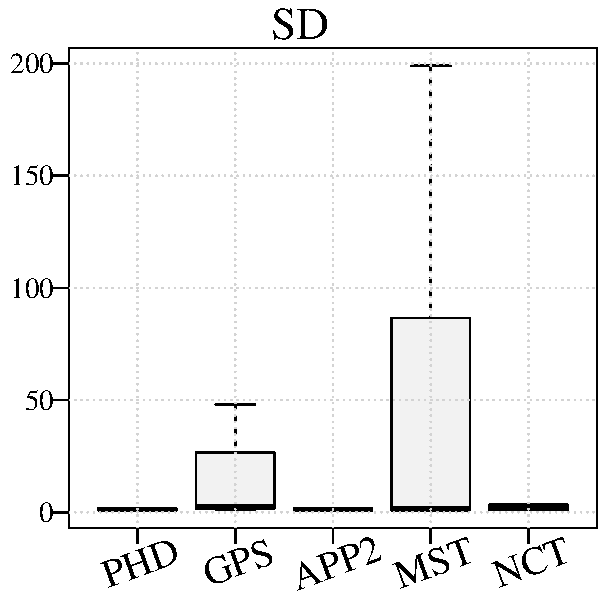
\includegraphics[width=0.31\columnwidth]{./fig/sd_opf} &% ./fig/compare/opf/sd
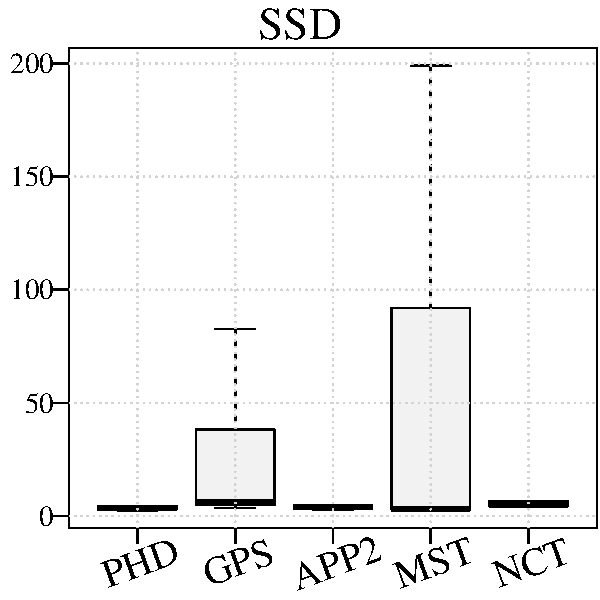
\includegraphics[width=0.31\columnwidth]{./fig/ssd_opf} &% ./fig/compare/opf/ssd
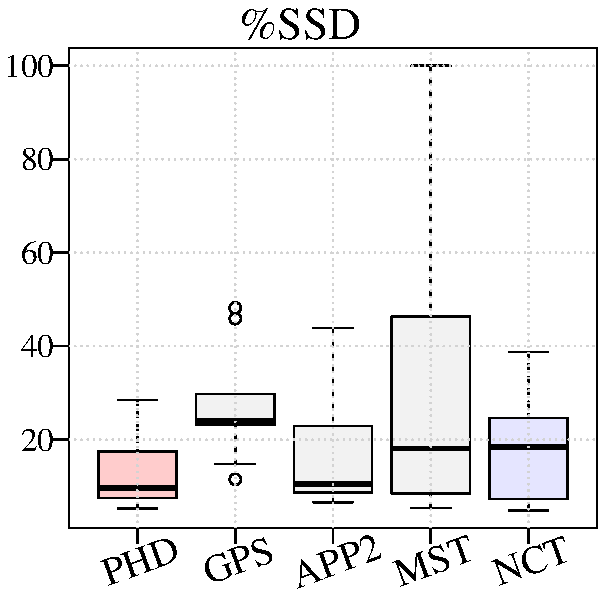
\includegraphics[width=0.31\columnwidth]{./fig/pssd_opf} \\% ./fig/compare/opf/pssd
\end{tabular}
\caption{Performance comparison of our method with several other methods on the OPF data set. For each method and each measure, the plotted box indicates the 25-75 percentile, the horizontal bar indicates the median score, and the whiskers and outliers are drawn using the default settings of R.}
\label{fig:compare-opf}
\end{figure}

% ************************************************************************
\clearpage
\begin{figure}[!t]
\centering
\begin{tabular}{c@{\hspace{0.02\columnwidth}}c@{\hspace{0.02\columnwidth}}c}
\includegraphics[width=0.31\columnwidth]{./fig/p_saria} &% ./fig/compare/saria/p
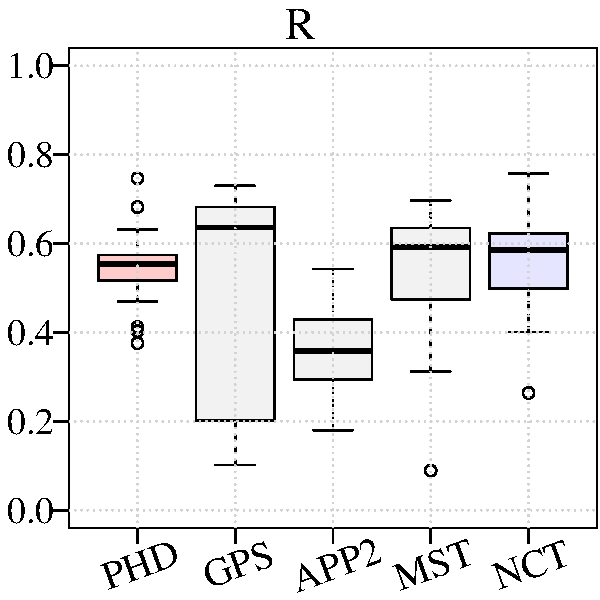
\includegraphics[width=0.31\columnwidth]{./fig/r_saria} &% ./fig/compare/saria/r
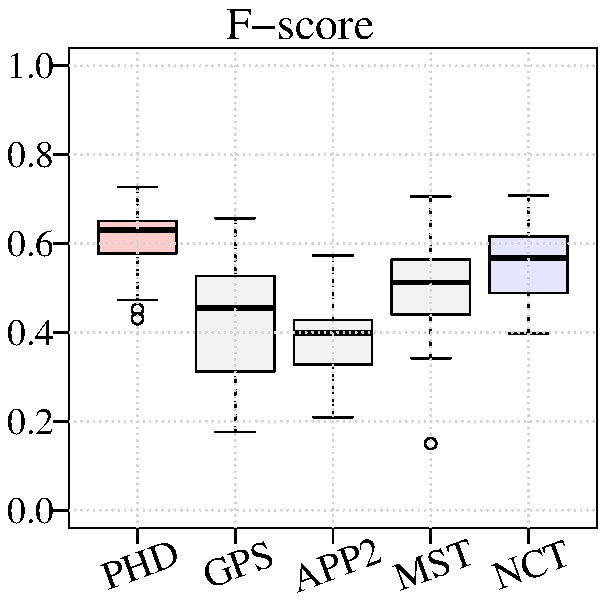
\includegraphics[width=0.31\columnwidth]{./fig/f_saria} \\[1ex]% ./fig/compare/saria/f
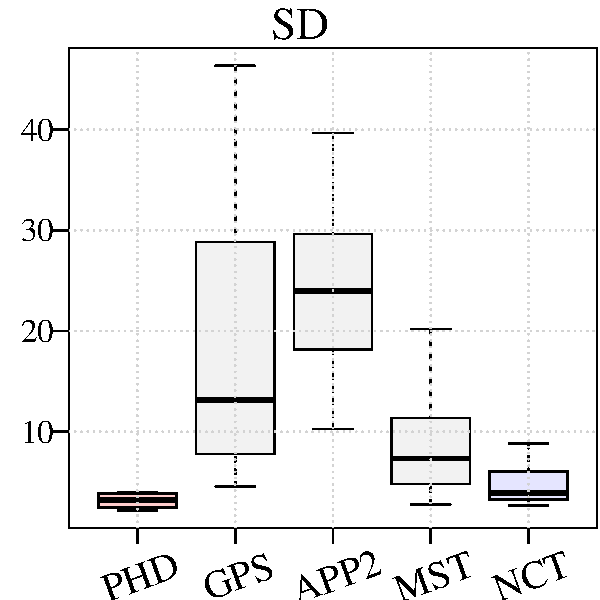
\includegraphics[width=0.31\columnwidth]{./fig/sd_saria} &% ./fig/compare/saria/sd
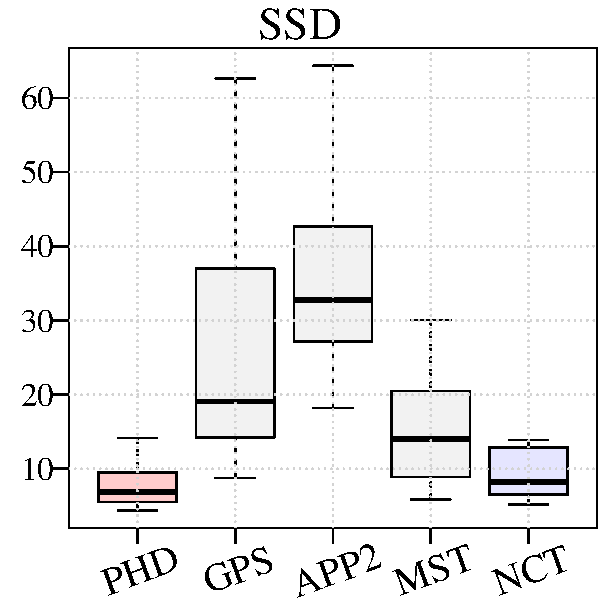
\includegraphics[width=0.31\columnwidth]{./fig/ssd_saria} &% ./fig/compare/saria/ssd
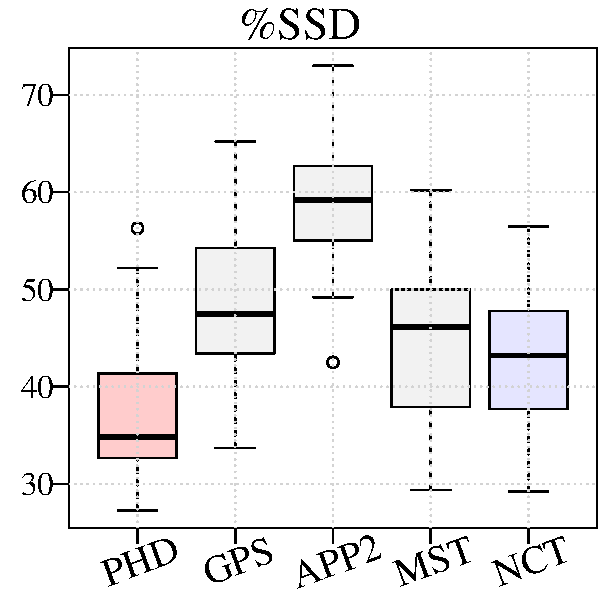
\includegraphics[width=0.31\columnwidth]{./fig/pssd_saria} \\% ./fig/compare/saria/pssd
\end{tabular}
\caption{Performance comparison of our method with several other methods on the HCN data set. For each method and each measure, the plotted box indicates the 25-75 percentile, the horizontal bar indicates the median score, and the whiskers and outliers are drawn using the default settings of R.}
\label{fig:compare-saria}
\end{figure}

% ************************************************************************
\clearpage
\begin{figure}[!t]
\centering
\begin{tabular}{r@{\hspace{0.02\columnwidth}}c@{\hspace{0.02\columnwidth}}c@{\hspace{0.02\columnwidth}}c}
Case: &

\includegraphics[align=c,width=0.15\columnwidth]{./fig/c2.compare/i1_inv} &

\includegraphics[align=c,width=0.15\columnwidth]{./fig/c2.compare/i2_inv} &

\includegraphics[align=c,width=0.15\columnwidth]{./fig/c2.compare/i3_inv}\\
PHD: &
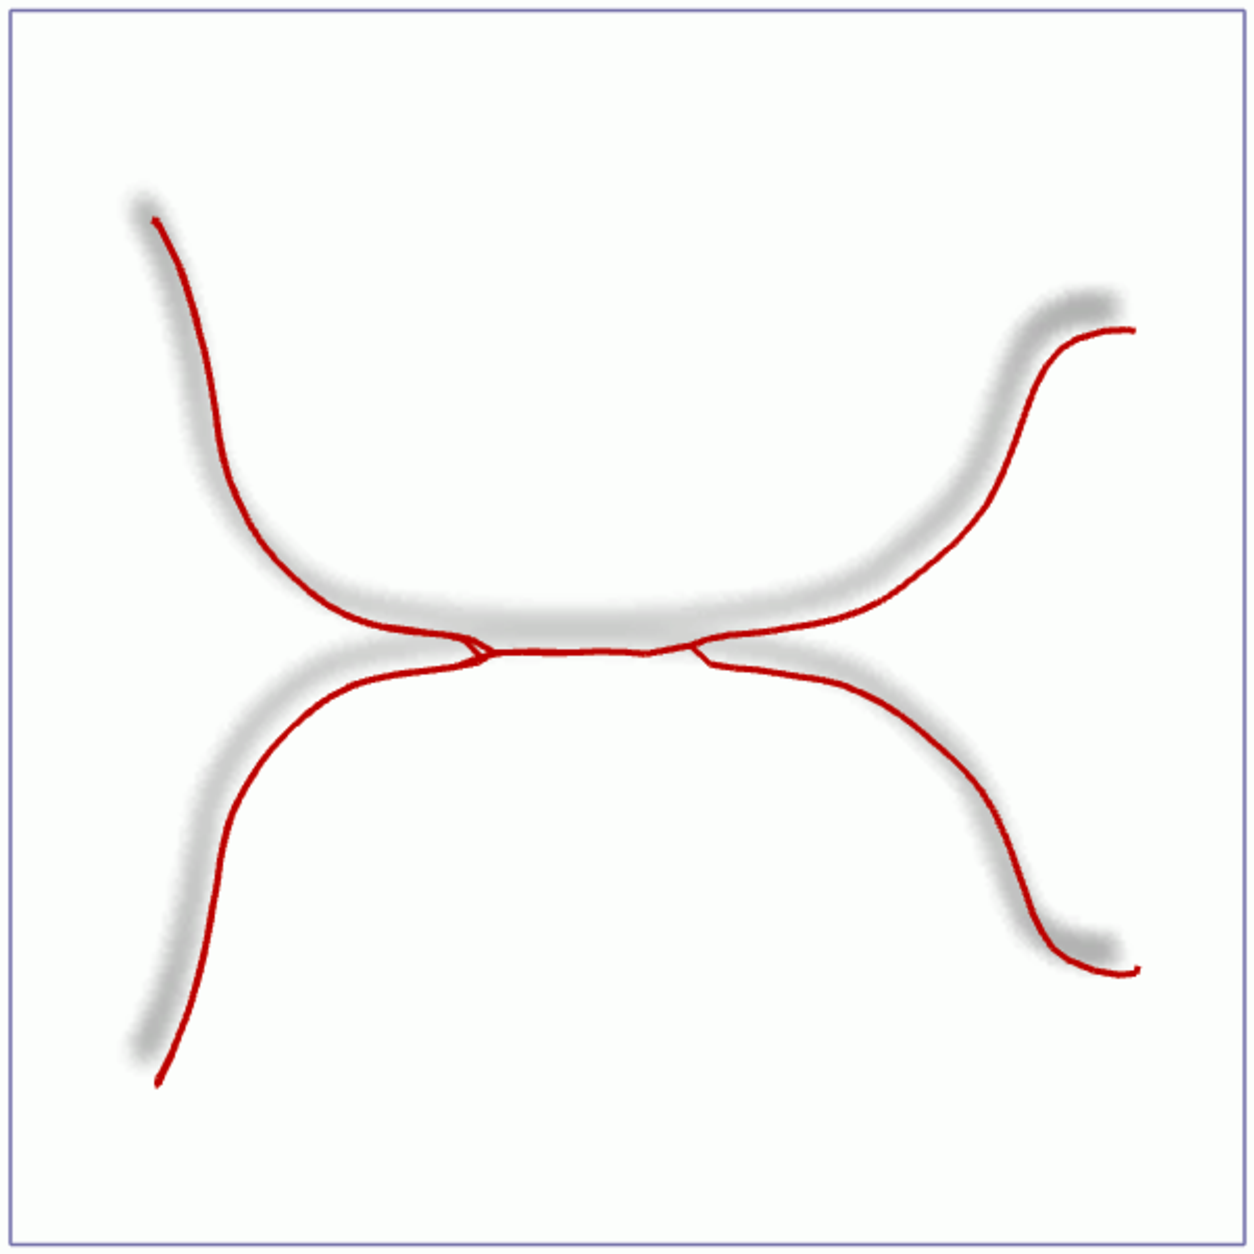
\includegraphics[align=c,width=0.2\columnwidth]{./fig/c2.compare/phd,i1,c0,s0} &
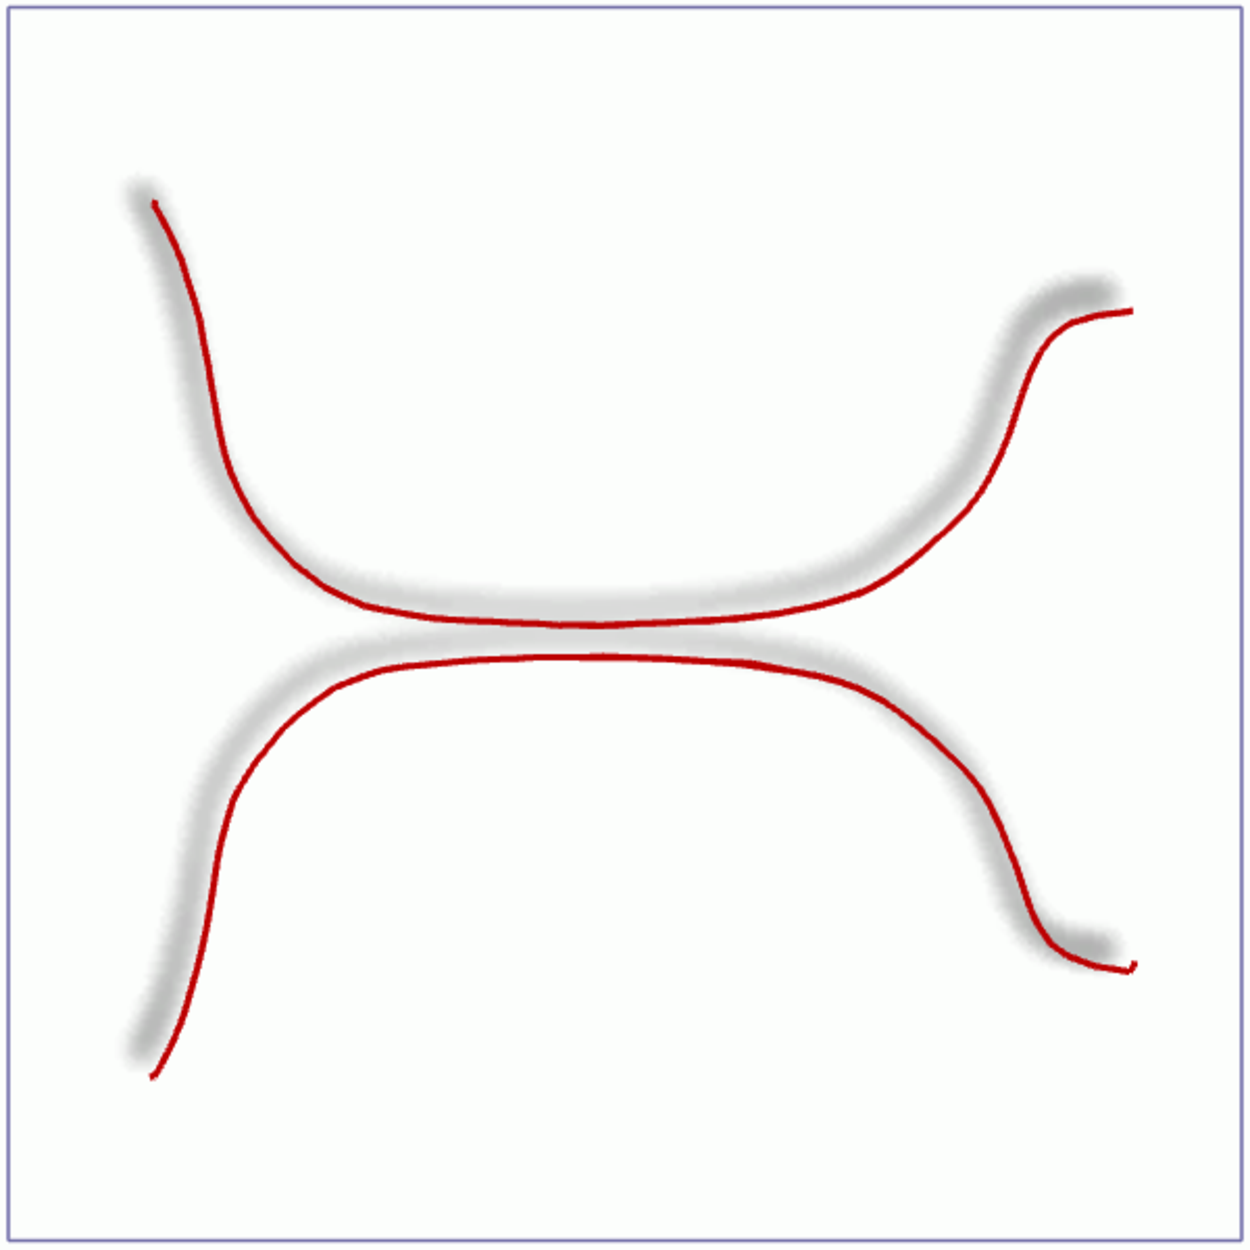
\includegraphics[align=c,width=0.2\columnwidth]{./fig/c2.compare/phd,i2,c0,s0} &
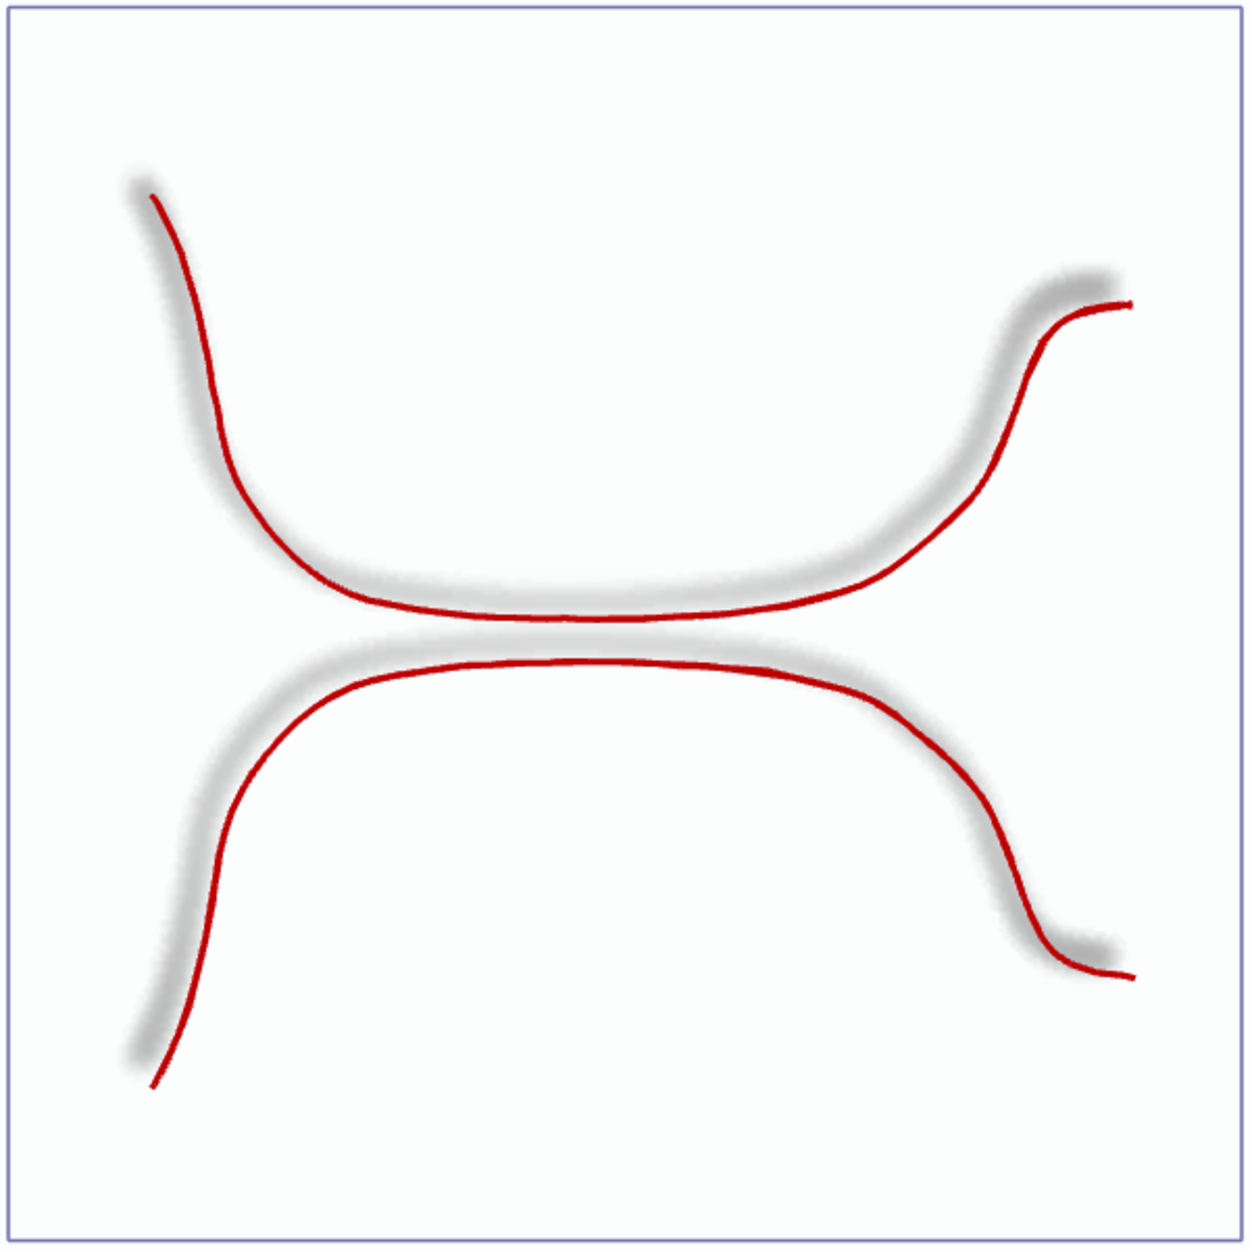
\includegraphics[align=c,width=0.2\columnwidth]{./fig/c2.compare/phd,i3,c0,s0} \\
GPS: &
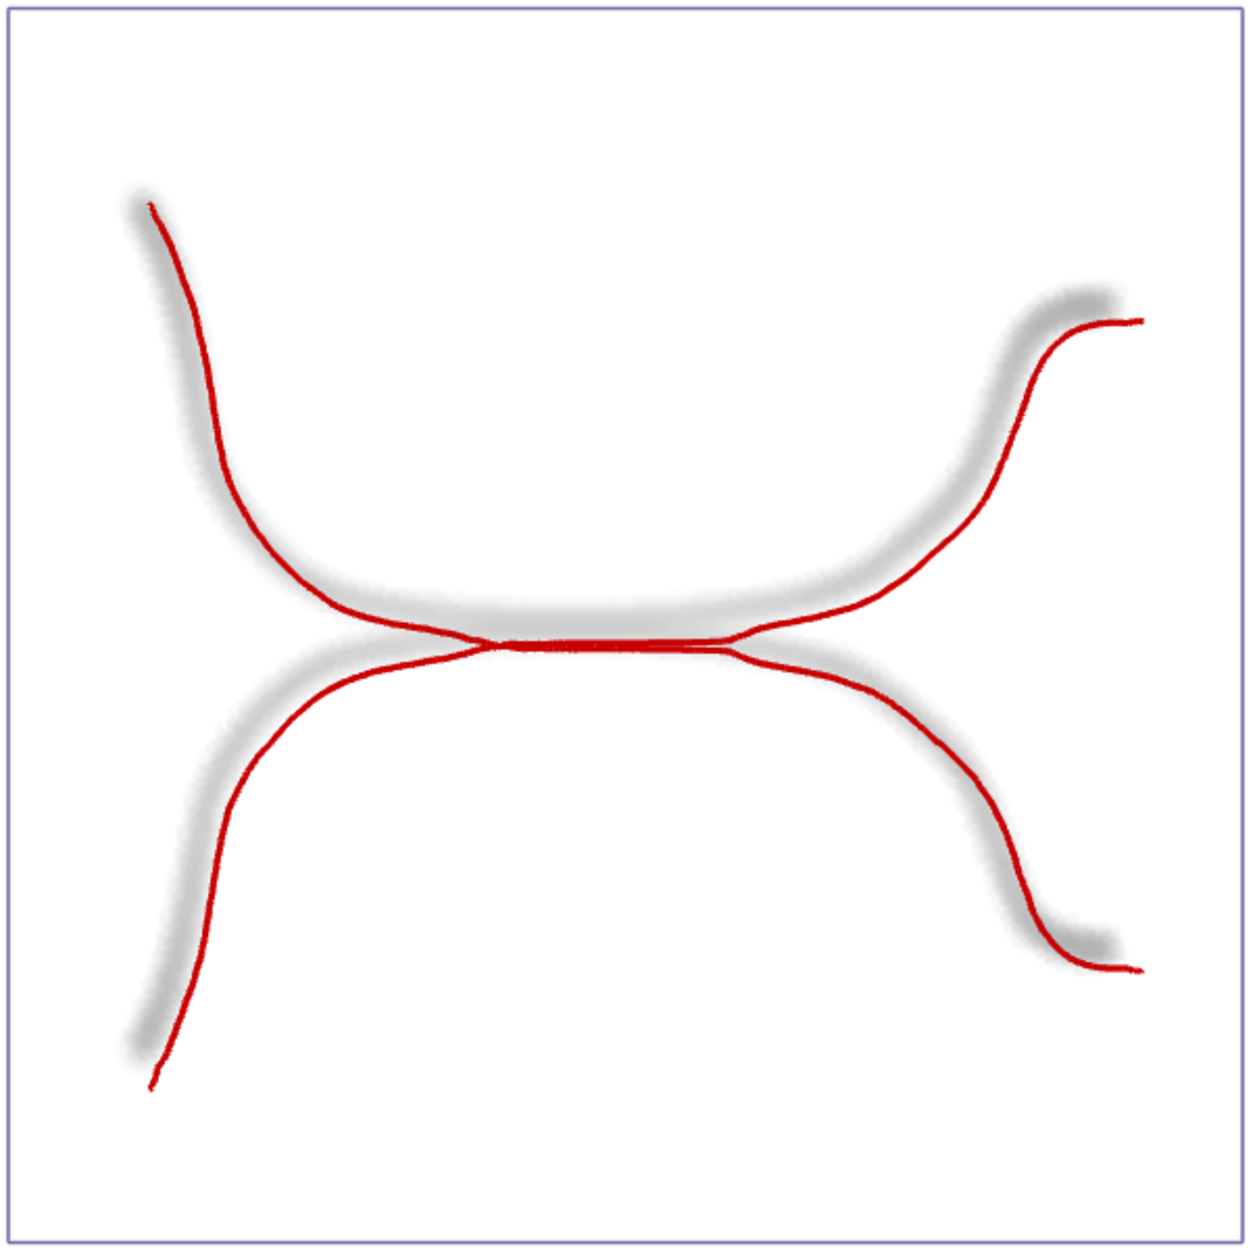
\includegraphics[align=c,width=0.2\columnwidth]{./fig/c2.compare/gps,i1} &
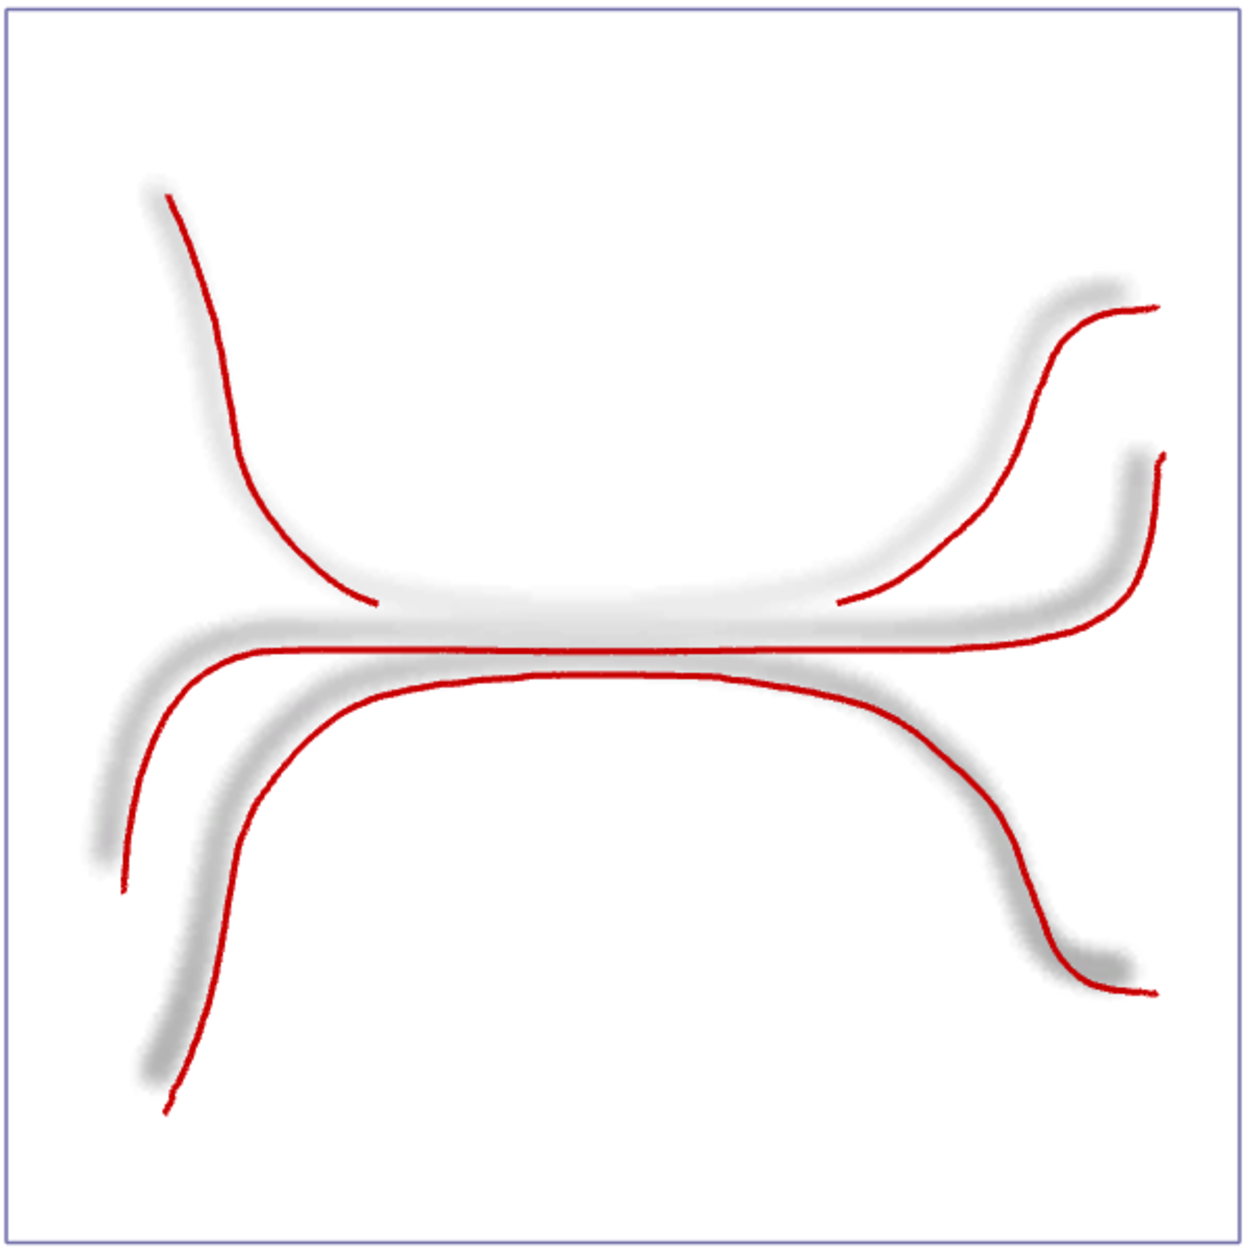
\includegraphics[align=c,width=0.2\columnwidth]{./fig/c2.compare/gps,i2} &
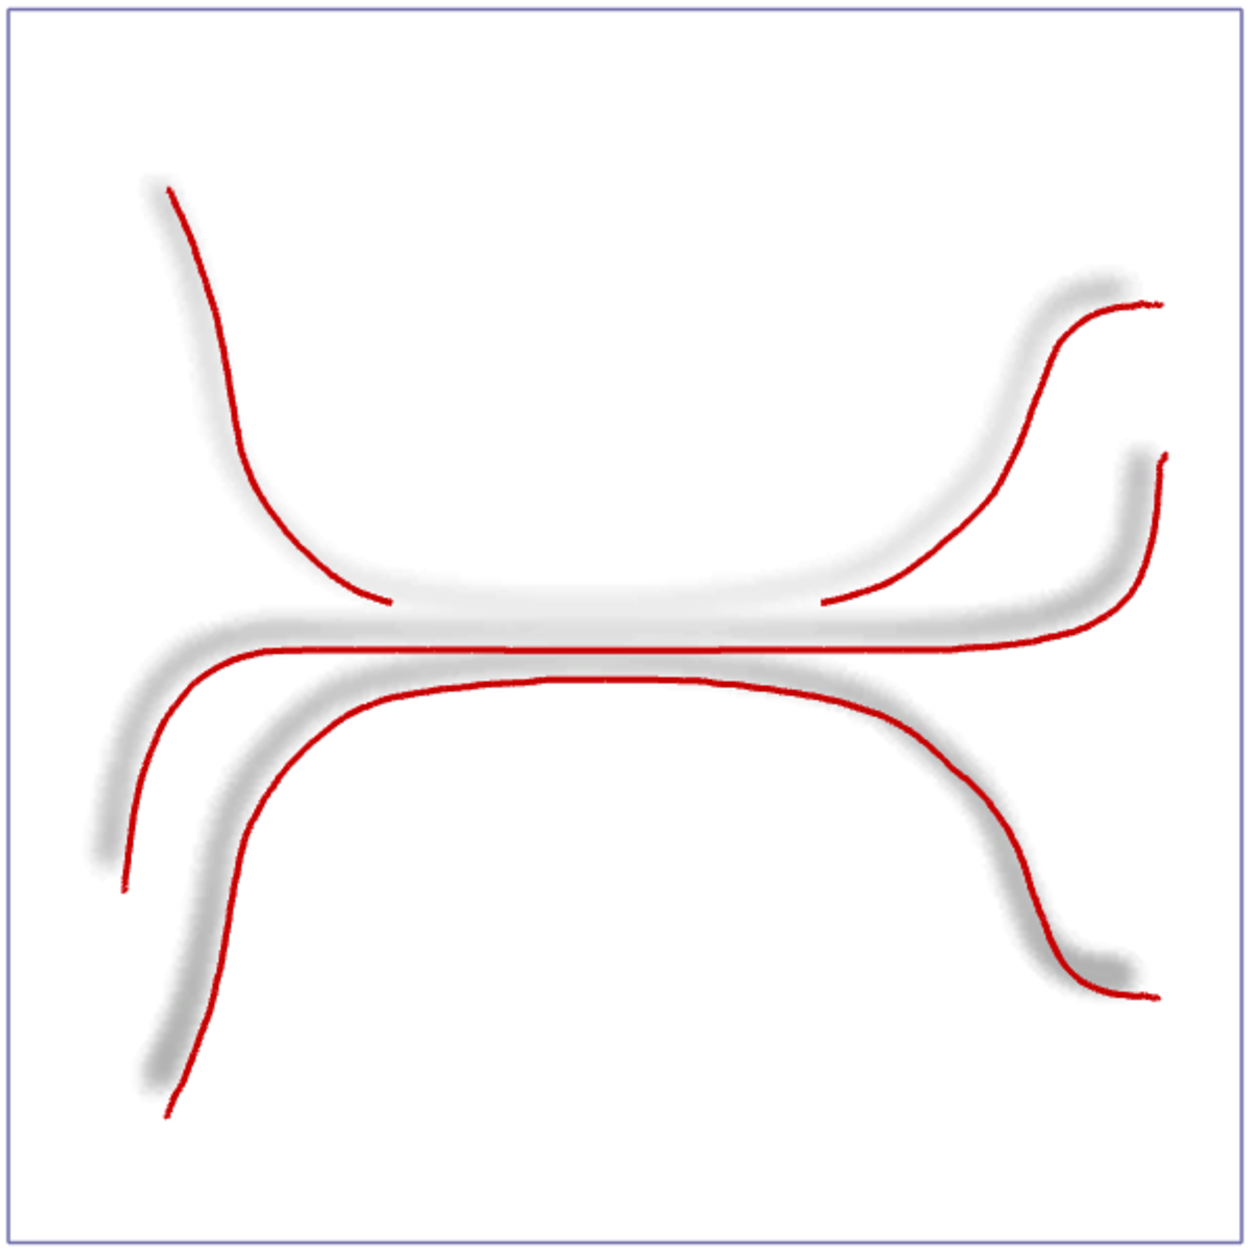
\includegraphics[align=c,width=0.2\columnwidth]{./fig/c2.compare/gps,i3} \\
APP2: &
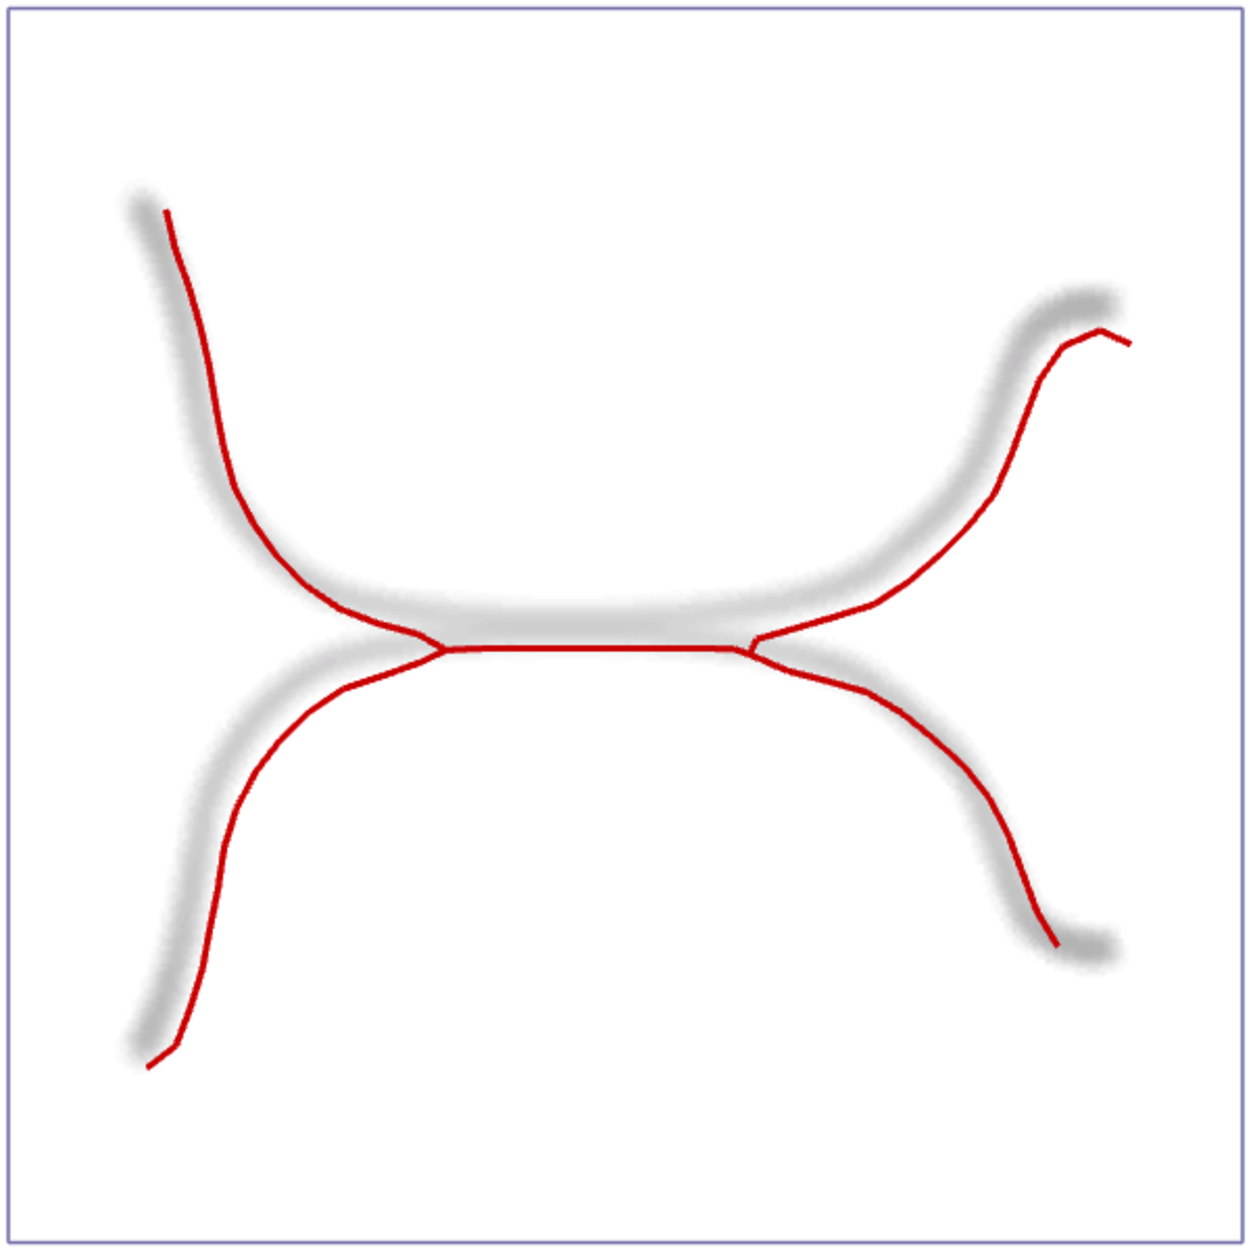
\includegraphics[align=c,width=0.2\columnwidth]{./fig/c2.compare/app2,i1} &
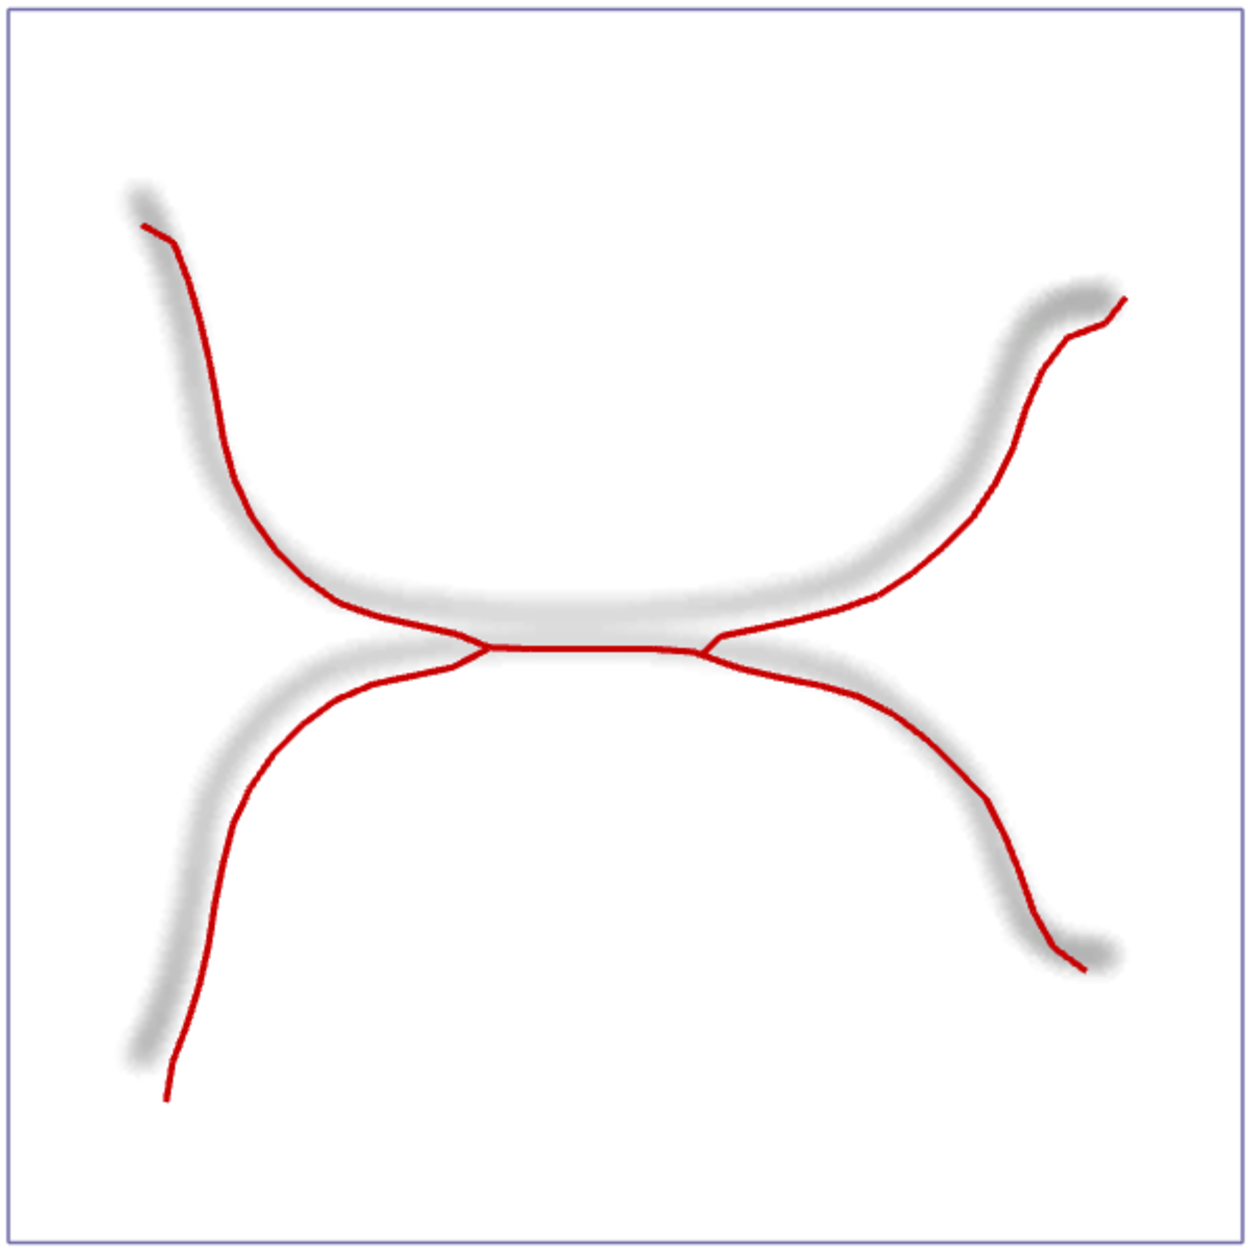
\includegraphics[align=c,width=0.2\columnwidth]{./fig/c2.compare/app2,i2} &
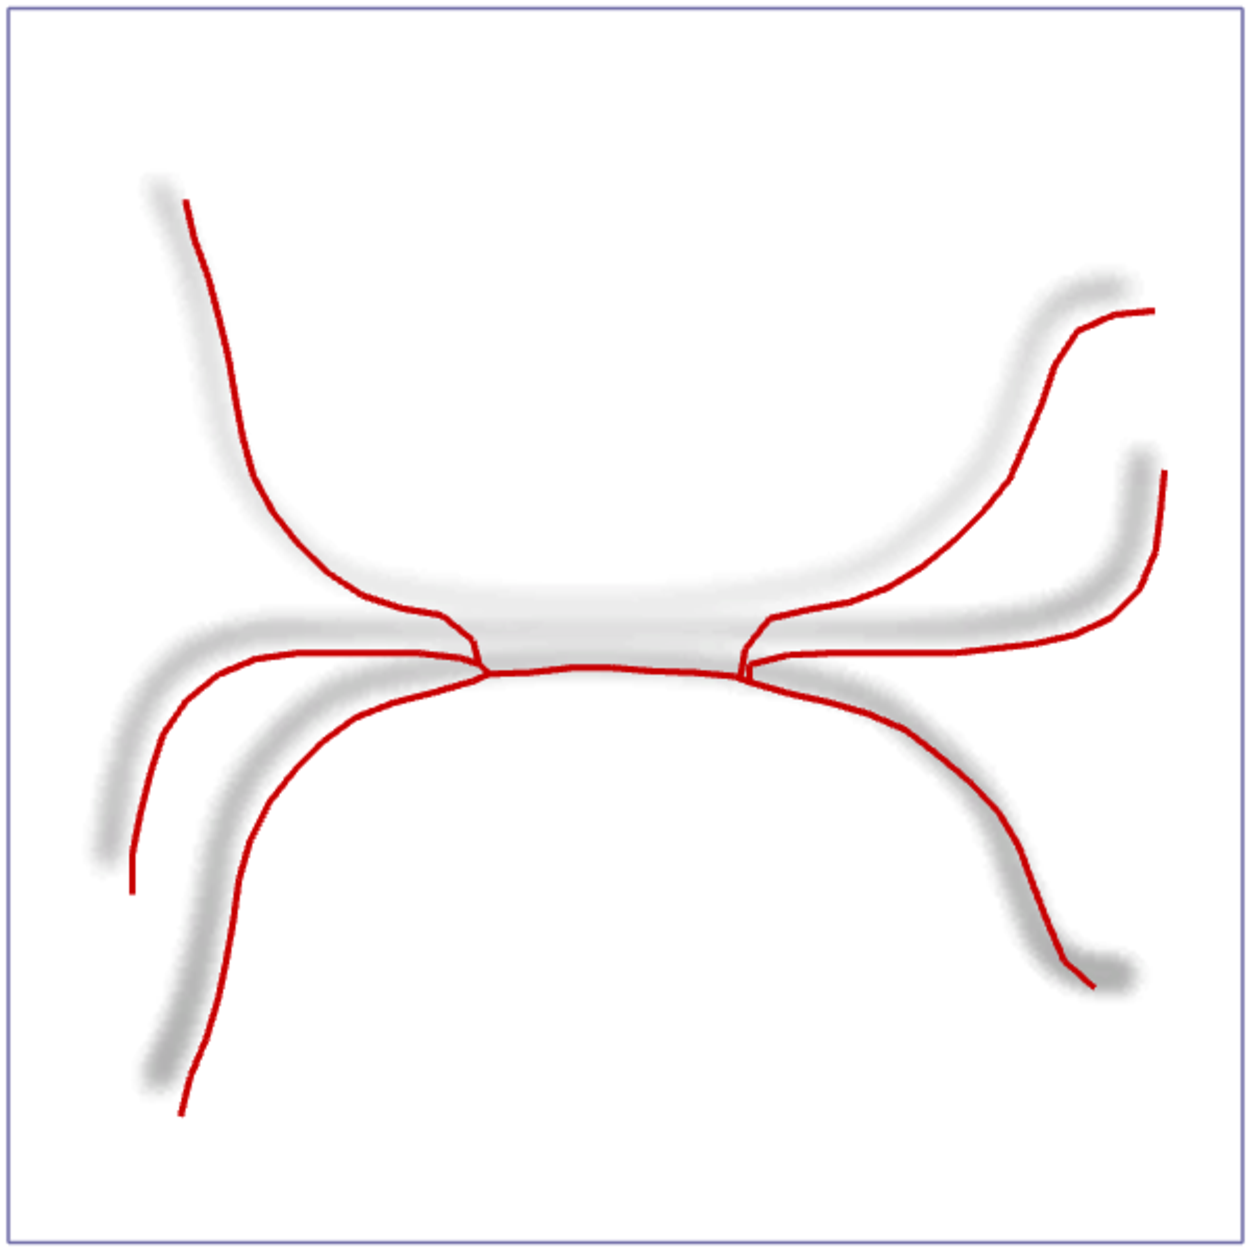
\includegraphics[align=c,width=0.2\columnwidth]{./fig/c2.compare/app2,i3} \\
MST: &
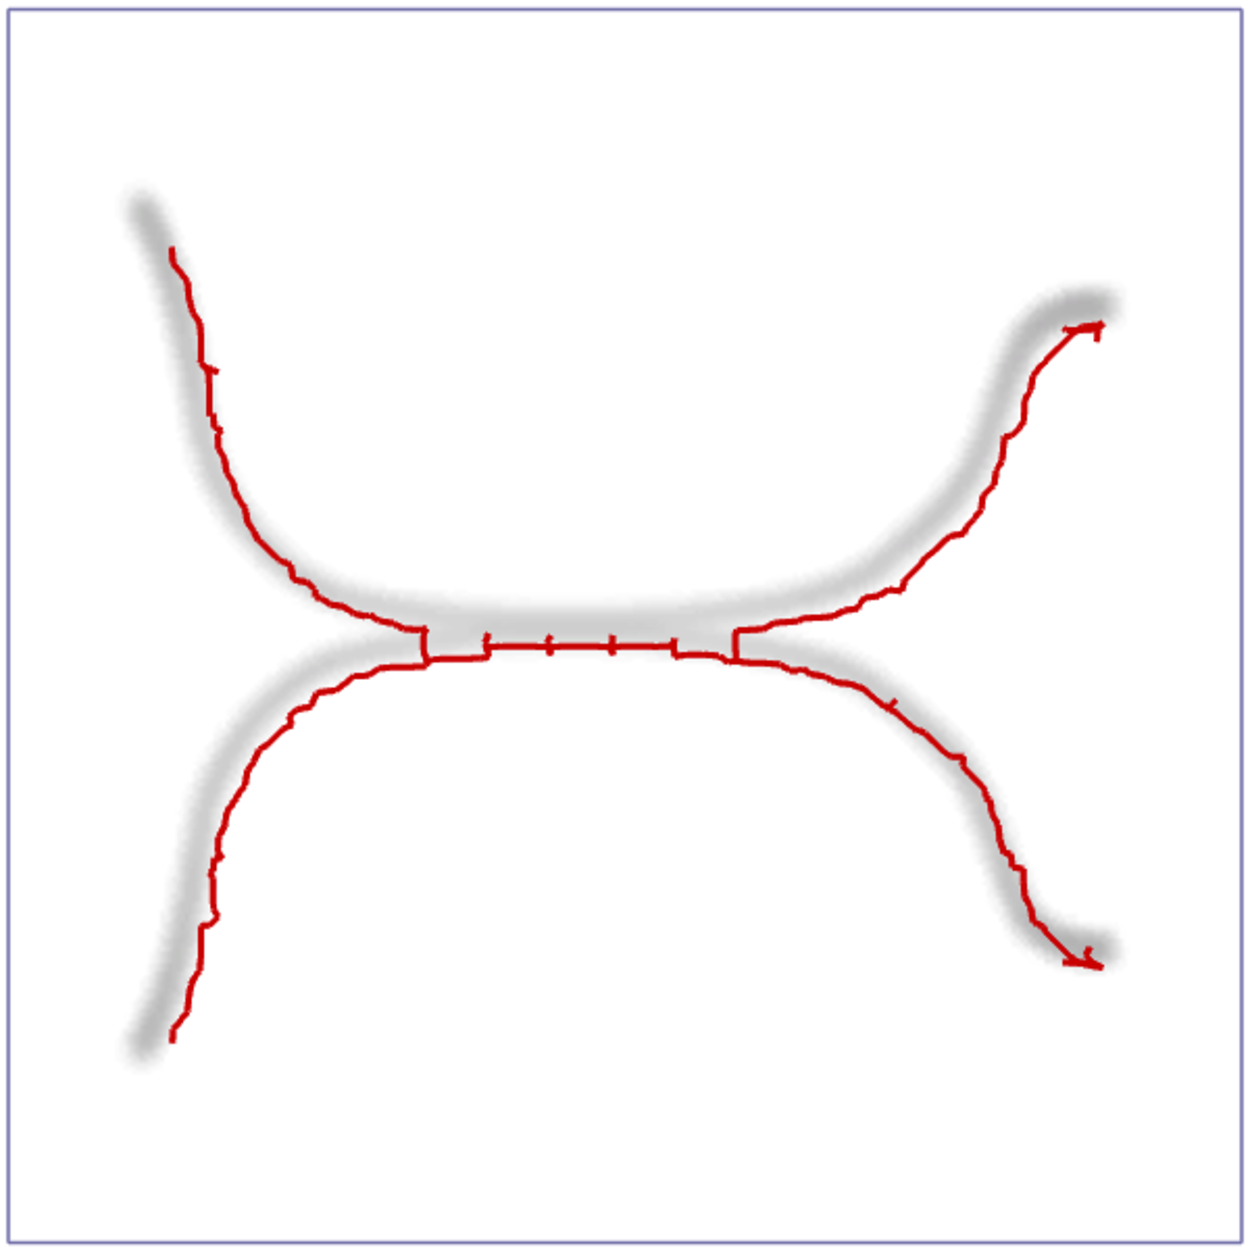
\includegraphics[align=c,width=0.2\columnwidth]{./fig/c2.compare/mst,i1} &
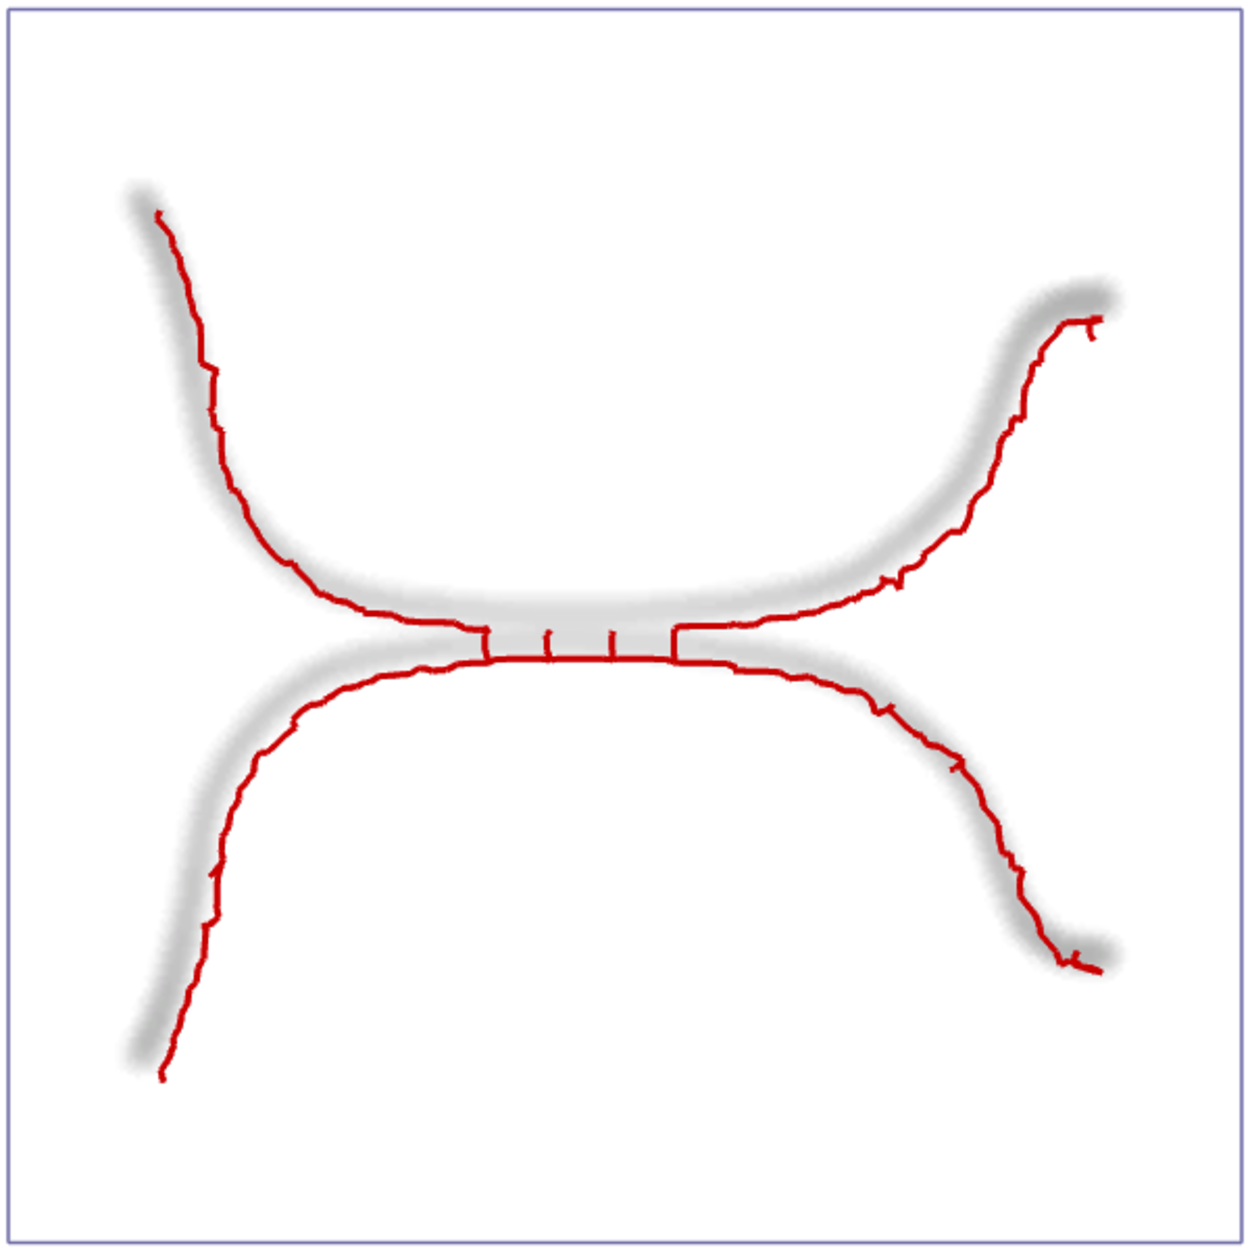
\includegraphics[align=c,width=0.2\columnwidth]{./fig/c2.compare/mst,i2} &
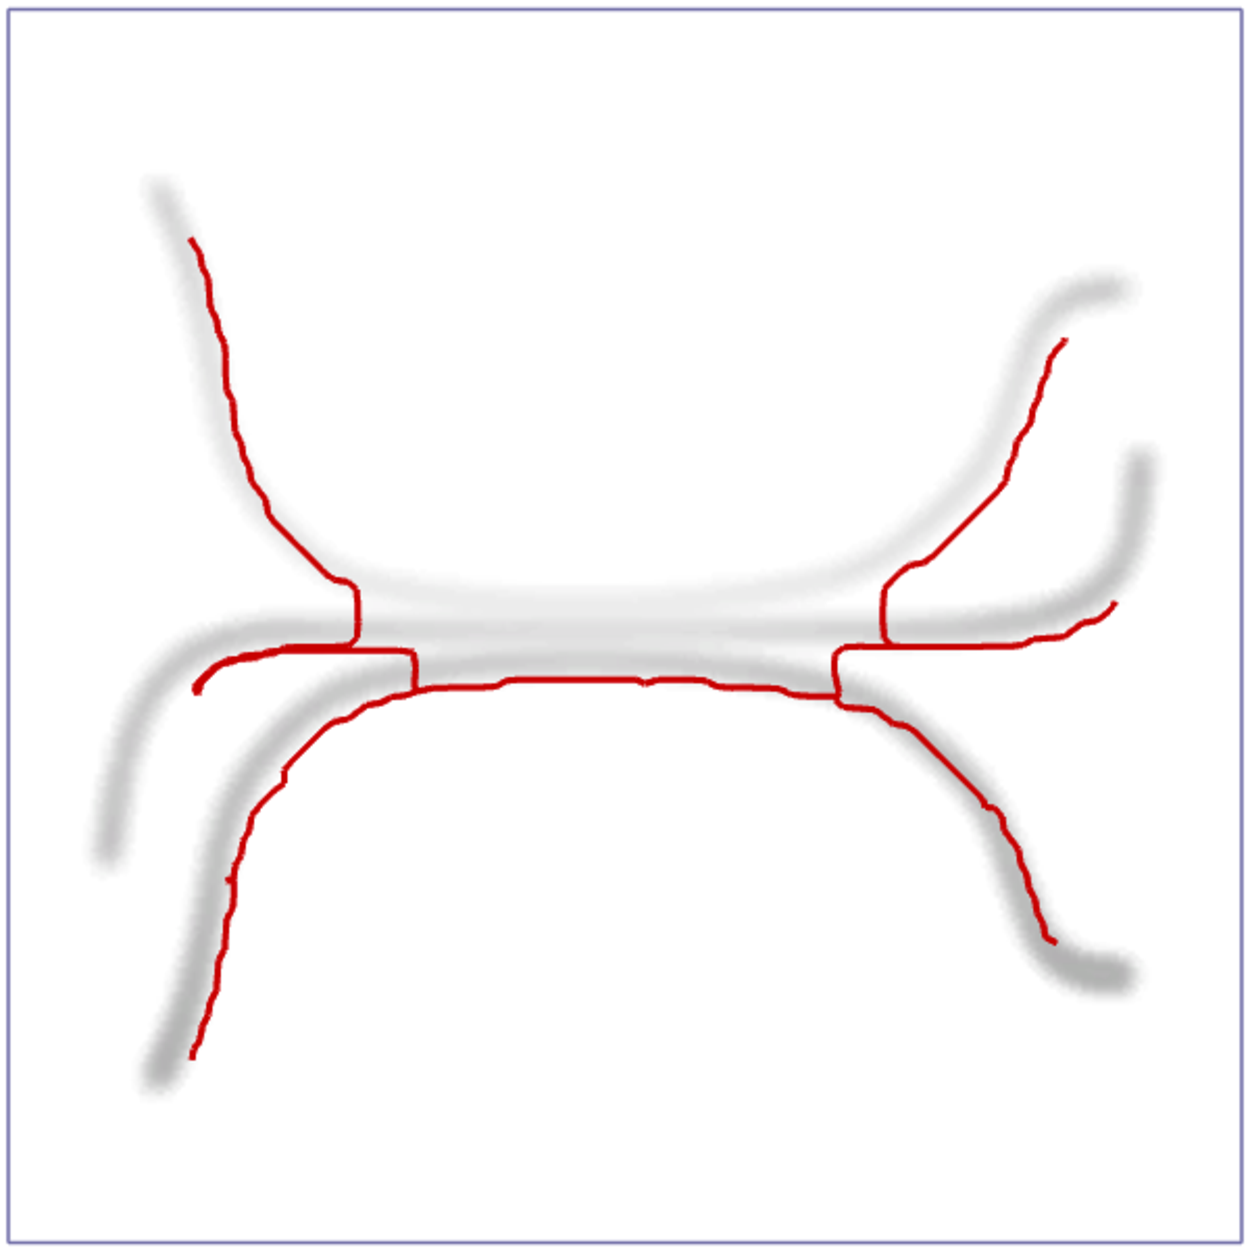
\includegraphics[align=c,width=0.2\columnwidth]{./fig/c2.compare/mst,i3} \\
\end{tabular}
\caption{Ability of the tested methods to separate two fibers of similar intensity and scale running closely in parallel. The examples show cases with gradually increasing distance between the fibers: overlap (left column), just separated (middle column), and clearly separated (right column). The tracing results of PHD, GPS, APP2, MST are overlaid (with slight offset) in red color.}
\label{fig:phd-advantage-2}
\end{figure}

% ************************************************************************
\clearpage
\begin{figure}[!t]
\centering
\begin{tabular}{c@{\hspace{0.02\columnwidth}}c@{\hspace{0.02\columnwidth}}c@{\hspace{0.02\columnwidth}}c}
%\multicolumn{4}{c}{\includegraphics[align=c,width=0.2\columnwidth]{./fig/test2d.compare/i}}\\
Case: &
\includegraphics[align=c,width=0.15\columnwidth]{./fig/c3.compare/i1_inv} &
\includegraphics[align=c,width=0.15\columnwidth]{./fig/c3.compare/i2_inv} &
\includegraphics[align=c,width=0.15\columnwidth]{./fig/c3.compare/i3_inv}\\
PHD: &
\includegraphics[align=c,width=0.2\columnwidth]{./fig/c3.compare/phd,i1,c0,s0} &
\includegraphics[align=c,width=0.2\columnwidth]{./fig/c3.compare/phd,i2,c0,s0} &
\includegraphics[align=c,width=0.2\columnwidth]{./fig/c3.compare/phd,i3,c0,s0} \\
GPS: &
\includegraphics[align=c,width=0.2\columnwidth]{./fig/c3.compare/gps,i1} &
\includegraphics[align=c,width=0.2\columnwidth]{./fig/c3.compare/gps,i2} &
\includegraphics[align=c,width=0.2\columnwidth]{./fig/c3.compare/gps,i3} \\
APP2: &
\includegraphics[align=c,width=0.2\columnwidth]{./fig/c3.compare/app2,i1} &
\includegraphics[align=c,width=0.2\columnwidth]{./fig/c3.compare/app2,i2} &
\includegraphics[align=c,width=0.2\columnwidth]{./fig/c3.compare/app2,i3} \\
MST: &
\includegraphics[align=c,width=0.2\columnwidth]{./fig/c3.compare/mst,i1} &
\includegraphics[align=c,width=0.2\columnwidth]{./fig/c3.compare/mst,i2} &
\includegraphics[align=c,width=0.2\columnwidth]{./fig/c3.compare/mst,i3} \\
\end{tabular}
\caption{Ability of the tested methods to separate three fibers with different intensity and scale running closely in parallel. The examples show cases with gradually increasing distance between the fibers: overlap (left column), just separated (middle column), and clearly separated (right column). The tracing results of PHD, GPS, APP2, MST are overlaid (with slight offset) in red color.}
\label{fig:phd-advantage-3}
\end{figure}

% ************************************************************************
\end{document}
% ************************************************************************